\ylDisplay{Kaheksa} % Ülesande nimi
{Tundmatu autor} % Autor
{lõppvoor} % Voor
{2016} % Aasta
{P 9} % Ülesande nr.
{3} % Raskustase
{
% Teema: Elektriõpetus

\ifStatement
Juku paigutab takisteid takistusega $R$ number $8$ kuju järgi, nagu näidatud joonisel. Kõik takistid, millel on üks ühine punkt, on elektriliselt ühendatud. Juku mõõdab kõikvõimalike punktide vahel takistust. Millise vähima väärtuse ja milliste punktide vahel ta saab? Lahenduses vaadake läbi kõik võimalikud juhud. 
\begin{center}
	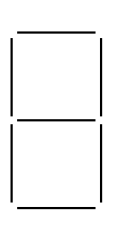
\includegraphics[width=0.5\linewidth]{2016-v3p-09-yl.png}
\end{center}
\fi

\ifHint
Tehes skeemis ühe takistuse takistust väiksemaks, siis kogutakistus kas väheneb või jääb samaks.
\fi

\ifSolution
\begin{center}
	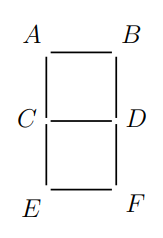
\includegraphics[width=0.5\linewidth]{2016-v3p-09-lah1.png}
\end{center}
Skeemi vaadates pakume, et kõige väiksem takistus on punktide $C$ ja $D$ vahel, kuna nende vahel on otseühendus ühe takistiga ja veel lisaks rööbiti kaks haru. Paralleelsete ühenduse korral on kogutakistus väiksem kõige väiksema haru takistusest ehk antud juhul peab see tulema väiksem kui $R$. Arvutame selle takistuse välja:
\begin{center}
$\frac{1}{R_{CD}} = \frac{1}{R} + \frac{1}{3R}+\frac{1}{3R}$ $\Rightarrow$  $R_{CD} = \frac{3}{5}R$.
\end{center}
Kõik teised kaks punkti, mida saame valida, sisaldavad ühte nurgapunkti. Et vältida sama takistuse mitu korda analüüsimist ja kuna kujund on igast nurgast vaadatuna samasugune, vaatleme takistusi punkti $A$ ja teiste punktide vahel. 
Takistuste hindamiseks asendame takistid $R_{CD}$, $R_{CE}$, $R_{EF}$ ja $R_{DF}$ nulltakistite ehk lihtsalt juhtmetega. Vastavalt vihjele niiviisi tehes kogutakistus kahe suvalise punkti vahel ei lähe suuremaks. Sisuliselt ühendame punktid $C$, $D$, $E$ ja $F$ kokku. Sellelt skeemilt näeme, et mõõtes kogutakistust A ja suvalise teise punkti X vahel, on meil alati rööbiti takistused R ja 2R ning takistus tuleb sama. Seega tähistame teist punkti X-ga. 
\begin{center}
	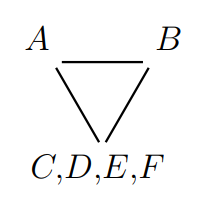
\includegraphics[width=0.5\linewidth]{2016-v3p-09-lah2.png}
\end{center}
Uuel skeemil tuleb kogutakistuseks:
\begin{center}
$\frac{1}{R'_{AX}} = \frac{1}{R} + \frac{1}{2R}$  $\Rightarrow$ $\frac{2}{3} R$
\end{center}
Näeme, et
\begin{center}
$\frac{1}{R'_{AX}} = \frac{2}{3} R =\frac{10}{15} R > \frac{9}{15}R = \frac{3}{5}R = R_{CD}$ $\Rightarrow$ $R'_{AX} > R_{CD}$.
\end{center}
Kuna vihje järgi on takistus $R'_{AX}$ väiksem või võrdne kogutakistusega $R_{AX}$ punkti $A$ ja vastava punkti vahel originaalses skeemis (sest vähendasime osasid takistusi nullini), saame, et 
\begin{center}
$R_{AX} \geq R'_{AX} > R_{CD}$ $\Rightarrow$ $R_{AX} > R_{CD}$.
\end{center}
Seega oleme tõestanud, et punktide $C$ ja $D$ vahel mõõdetud takistus $R_{CD}$ on kõige väiksem.
\fi
}